\documentclass[11pt]{article}
\usepackage[scaled=0.92]{helvet}
\usepackage{geometry}
\geometry{letterpaper,tmargin=1in,bmargin=1in,lmargin=1in,rmargin=1in}
\usepackage[parfill]{parskip} % Activate to begin paragraphs with an empty line rather than an indent %\usepackage{graphicx}
\usepackage{amsmath,amssymb, mathrsfs,  mathtools, dsfont}
\usepackage{tabularx}
\usepackage[font=footnotesize,labelfont=bf]{caption}
\usepackage{graphicx}
\usepackage{xcolor}
\usepackage{tikz-cd}
%\usepackage[linkbordercolor ={1 1 1} ]{hyperref}
%\usepackage[sf]{titlesec}
\usepackage{natbib}
\usepackage{../../Tianpei_Report}

%\usepackage{appendix}
%\usepackage{algorithm}
%\usepackage{algorithmic}

%\renewcommand{\algorithmicrequire}{\textbf{Input:}}
%\renewcommand{\algorithmicensure}{\textbf{Output:}}



\begin{document}
\title{Lecture 4: Compactness in Function Spaces}
\author{ Tianpei Xie}
\date{Dec. 1st., 2022 }
\maketitle
\tableofcontents
\newpage
\section{Complete Metric Spaces and Function Spaces}
\subsection{Complete Metric Space}
\begin{itemize}
\item \begin{definition} (\emph{\textbf{Cauchy Net in Topological Vector Space}})\\
A \emph{net}  $\set{x_\alpha}_{\alpha \in I}$ in \emph{\textbf{toplogocial vector space}} $X$ is called \underline{\emph{\textbf{Cauchy}}} if the net $\set{x_{\alpha} - x_{\beta}}_{(\alpha, \beta) \in I \times I}$
\emph{\textbf{converges} to zero}. (Here $I \times I$ is \emph{\textbf{directed}} in the usual way: $(\alpha, \beta) \prec (\alpha', \beta')$ if and only if $\alpha \prec \alpha'$ and $\beta \prec \beta'$.) 
\end{definition}

\item \begin{definition} (\emph{\textbf{Completeness}})\\
A toplogocial vector space $X$ is \emph{\textbf{complete}} if every Cauchy net converges.
\end{definition}

\item \begin{proposition} (\textbf{Complete First Countable Topological Vector Space})\\
If $X$ is a \textbf{first-countable topological vector space} and every \textbf{Cauchy sequence} in $X$ converges, then every \textbf{Cauchy net} in $X$ converges.
\end{proposition}

\item \begin{proposition} (\textbf{Completeness of Euclidean Space}) \citep{munkres2000topology} \\
Euclidean space $\bR^k$ is \textbf{complete} in either of its usual \textbf{metrics}, the \textbf{euclidean metric} $d$ or the \textbf{square metric} $\rho$.
\end{proposition}

\item \begin{lemma} (\textbf{Convergence in Product Space is Weak Convergence}) \citep{munkres2000topology} \\
Let $X$ be the product space $X = \prod_{\alpha}X_{\alpha}$; let $x_n$ be a sequence of points of $X$. Then $x_n \rightarrow x$ if and only if $\pi_{\alpha}(x_n) \rightarrow  \pi_{\alpha}(x)$ for each $\alpha$.
\end{lemma}

\item \begin{proposition} (\textbf{Completeness of Countable Product Space}) \citep{munkres2000topology} \\
There is a metric for the product space $\bR^{\omega}$ relative to which $\bR^{\omega}$ is \textbf{complete}.
\end{proposition}

\item \begin{definition} (\emph{\textbf{Uniform Metric in Function Space}})\\
Let $(Y, d)$ be a metric space; let $\bar{d}(a, b) = \min\{d(a, b), 1\}$ be the \emph{\textbf{standard bounded metric}} on $Y$ derived from $d$. If $x = (x_{\alpha})_{\alpha \in J}$ and  $y = (y_{\alpha})_{\alpha \in J}$ are points of the cartesian product $Y^J$, let
\begin{align*}
\bar{\rho}(x, y) = \sup\set{\bar{d}(x_{\alpha}, y_{\alpha}): \alpha \in J}.
\end{align*}
It is easy to check that $\bar{\rho}$ is a metric; it is called \underline{\emph{\textbf{the uniform metric}}} on $Y^J$ corresponding to the metric $d$ on $Y$.

Note that \emph{\textbf{the space of all functions} $f: J \rightarrow Y$}, \emph{\textbf{denoted}} as $Y^{J}$, is a subset of the product space $J \times Y$. We can define uniform metric in the function space: if $f$, $g : J \rightarrow Y$, then
\begin{align*}
\bar{\rho}(f, g) = \sup\set{\bar{d}(f(\alpha), g(\alpha)): \alpha \in J}.
\end{align*}
\end{definition}

\item \begin{proposition} (\textbf{Completeness of Function Space  Under Uniform Metric}) \citep{munkres2000topology} \\
If the space $Y$ is \textbf{complete} in the metric $d$, then the space $Y^J$ is \textbf{complete} in the \textbf{uniform metric} $\bar{\rho}$ corresponding to $d$.
\end{proposition}

\item \begin{definition} (\emph{\textbf{Space of Continuous Functions and Bounded Functions}})\\
Let $Y^{X}$ be  \emph{the space of all functions} $f: X \rightarrow Y$, where $X$ is a \emph{topological space} and $Y$ is a \emph{metric space with metric $d$}. Denote the \emph{\textbf{subspace}}  of $Y^X$ consisting of all \emph{\textbf{continuous functions} $f$} as $\cC(X, Y)$. 

Also denote \emph{the set  of all \textbf{bounded functions}} $f: X \rightarrow Y$ as $\cB(X, Y)$. (A function $f$ is said to be \emph{\textbf{bounded}} if its image $f(X)$ is a \emph{\textbf{bounded subset}} of \emph{the metric space $(Y, d)$}.) 
\end{definition}

\item \begin{proposition}  (\textbf{Completeness of $\cC(X, Y)$ and   $\cB(X, Y)$  Under Uniform Metric}) \citep{munkres2000topology} \\
Let $X$ be a topological space and let $(Y, d)$ be a metric space. The set $\cC(X, Y)$ of \textbf{continuous} functions is \textbf{closed} in $Y^X$ under the \textbf{uniform metric}. So is the set $\cB(X, Y)$ of \textbf{bounded functions}. Therefore, if $Y$ is \textbf{complete}, these spaces are \textbf{complete} in the \textbf{uniform metric}.
\end{proposition}

\item \begin{definition} (\emph{\textbf{Sup Metric on Bounded Functions}})\\
If $(Y, d)$ is a metric space, one can define another metric \emph{on the set $\cB(X, Y)$ of \textbf{bounded functions}} from $X$ to $Y$ by the equation
\begin{align*}
\rho(x, y) = \sup\set{d(f(x), g(x)): x \in X}.
\end{align*}
It is easy to see that $\rho$ is well-defined, for the set $f(X) \cup g(X)$ is \emph{\textbf{bounded}} if both $f(X)$ and $g(X)$ are. The metric $\rho$ is called \underline{\emph{\textbf{the sup metric}}}.
\end{definition}

\item \begin{theorem} (\textbf{Existence of Completion}) \citep{munkres2000topology}\\
Let $(X, d)$ be a metric space. There is an \textbf{isometric embedding} of $X$ into a \textbf{complete} metric space.
\end{theorem}

\item \begin{definition} (\emph{\textbf{Completion}})\\
Let $X$ be a \emph{metric space}. If $h : X \rightarrow Y$ is an \textbf{\emph{isometric embedding}} of $X$ into a \emph{\textbf{complete} metric space} $Y$, then the \emph{\textbf{subspace}} $h(X)$ of $Y$ is a \emph{complete metric space}. It is called \underline{\emph{\textbf{the completion of $X$}}}.
\end{definition}
\end{itemize}

\subsection{Compactness in Metric Spaces}
\begin{itemize}
\item \begin{remark} (\emph{\textbf{Compactness} and \textbf{Completeness}})\\
How is \emph{\textbf{compactness}} of a metric space $X$ related to \emph{\textbf{completeness}} of $X$? 

The followings is from \emph{the sequential compactness} and definition of \emph{completeness}:
\begin{proposition}
Every \textbf{compact} metric space is \textbf{complete}.
\end{proposition}
The \emph{converse} does not hold -- \emph{\textbf{a complete metric space need not be compact}}. It is reasonable to ask what \emph{\textbf{extra condition}} one needs to impose on a complete space to be assured of its compactness.
Such a condition is the one called \emph{total boundedness}.
\end{remark}

\item \begin{definition} (\emph{\textbf{Total Boundedness}})\\
A metric space $(X, d)$ is said to be \underline{\emph{\textbf{totally bounded}}} if for every $\epsilon > 0$, there is a \emph{\textbf{finite covering} of $X$ by \textbf{$\epsilon$-balls}}.
\end{definition}

\item \begin{theorem} \citep{munkres2000topology}\\
A metric space $(X, d)$ is \textbf{compact} \underline{if and only if} it is \textbf{complete} and \textbf{totally bounded}.
\end{theorem}

\item \begin{remark}
We now apply this result to find \emph{\textbf{the compact subspaces}} of the space $\cC(X, \bR^n)$, \emph{in the \textbf{uniform topology}}. We know that a subspace of $\bR^n$ is compact if and only if it is \emph{\textbf{closed}} and \emph{\textbf{bounded}}. 

One might hope that an analogous result holds for $\cC(X, \bR^n)$. \emph{\textbf{But}} it does not, even if $X$ is \emph{compact}. One needs to assume that the subspace of $\cC(X, \bR^n)$ satisfies \emph{an \textbf{additional condition}}, called \emph{\textbf{equicontinuity}}. 
\end{remark}

\item \begin{definition}  (\emph{\textbf{Equicontinuity}}) \citep{reed1980methods, munkres2000topology} \\
Let $(Y, d)$ be a \emph{metric space}. Let $\srF$ be a \emph{subset} of the function space $\cC(X, Y)$ (i.e. $f \in \srF$ is continuous). If $x_0 \in X$, \emph{the set $\srF$ of functions} is said to be \underline{\emph{\textbf{equicontinuous at $x_0$}}} if given $\epsilon >0$, there is a neighborhood $U$ of $x_0$ such that \emph{for all $x \in U$} and \underline{\emph{\textbf{all $f \in \srF$}}},
\begin{align*}
d(f(x), f(x_0)) < \epsilon.
\end{align*}
If the set $\srF$ is \emph{equicontinuous} at $x_0$ for each $x_0 \in X$, it is said simply to be \underline{\emph{\textbf{equicontinuous}}} or $\srF$ is an \underline{\emph{\textbf{equicontinuous family}}}.

We say $\srF$ is a \underline{\emph{\textbf{uniformly equicontinuous family}}} if and only if for all $\epsilon >0$, there exists $\delta > 0$ such that $d(f(x), f(x')) < \epsilon$ whenever $p(x, x') < \delta$ for all $x, x' \in X$ and \emph{\textbf{every $f \in \srF$}}.
\end{definition}

\item \begin{remark}
An \emph{equicontinuous family} of functions is \emph{a family of continuous functions}.
\end{remark}

\item \begin{remark}
\emph{\textbf{Continuity}} of the function $f$ at $x_0$ means that \emph{\textbf{given} $f$} and given $\epsilon >0$, there exists a neighborhood $U$ of $x_0$ such that $d(f(x), f(x_0)) < \epsilon$ for $x \in U$. 
\textbf{
\emph{\textbf{Equicontinuity}} of $\srF$ means that \emph{\textbf{a single neighborhood}} $U$ can be chosen that will \emph{}work for all the functions} $f$ in the collection $\srF$.
\end{remark}

\item \begin{lemma} (\textbf{Total Boundedness $\Rightarrow$ Equicontinuous}) \citep{munkres2000topology}\\ 
Let $X$ be a \textbf{space}; let $(Y, d)$ be a \textbf{metric} space. If the subset $\srF$ of $\cC(X, Y)$ is \textbf{totally bounded} under the \textbf{uniform metric} corresponding to $d$, then $\srF$ is \textbf{equicontinuous} under $d$.
\end{lemma}

\item \begin{lemma} (\textbf{Equicontinuous $+$ Compactness  $\Rightarrow$ Total Boundedness})  \citep{munkres2000topology}\\ 
Let $X$ be a space; let $(Y, d)$ be a metric space; assume $X$ and $Y$ are \textbf{compact}. If the subset $\srF$ of $\cC(X, Y)$ is \textbf{equicontinuous} under $d$, then $\srF$ is \textbf{totally bounded} under the \textbf{uniform} and \textbf{sup} metrics corresponding to $d$.
\end{lemma}


%\item \begin{proposition}
%Let $f_n$ be a sequence of functions from one metric space to another with the property that the family $\{f_n\}$ is \textbf{equicontinuous}. Suppose
%that $f_n(x) \rightarrow f(x)$ \textbf{pointwise} for each $x$. Then $f$ is \textbf{continuous}.
%\end{proposition}
%
%\item We see that \emph{\textbf{pointwise convergence}} on a \emph{\textbf{dense set}} combined with \emph{\textbf{equicontinuity}} implies \emph{\textbf{pointwise convergence everywhere}}.
%\begin{proposition} \citep{reed1980methods}\\
%Let $\{f_n\}$ be an \textbf{equicontinuous family} of functions from one metric space $(X, p)$ to another $(Y, d)$ with $Y$ complete. Suppose that for a \textbf{dense} set $D \subseteq X$, we know $f_{n}(x)$ converges for all $x \in D$. Then $f_{n}(x)$ converges for all $x \in X$.
%\end{proposition}
%
%\item The following shows that uniformly equicontinuous combined with pointwise convergence implies uniform convergence.
%\begin{proposition} \citep{reed1980methods}\\
%Let $\{f_n\}$ be a \textbf{uniformly equicontinuous family} of functions on $[0, 1]$. Suppose that $f_n(x) \rightarrow f(x)$ for each $x$ in $[0, 1]$. Then $f_n(x) \rightarrow f(x)$  \textbf{uniformly} in $x$.
%\end{proposition}
%
%\item \begin{remark}
%For functions on $[0, 1]$, \emph{every \textbf{equicontinuous family}} is \emph{\textbf{uniformly equicontinuous}}.
%\end{remark}

\item \begin{definition} (\emph{\textbf{Pointwise Bounded}})\\
If $(Y, d)$ is a \emph{metric space}, a \emph{subset} $\srF$ of $\cC(X, Y)$ is said to be \underline{\emph{\textbf{pointwise bounded}}} under $d$ if for each $x \in X$, the subset
\begin{align*}
F_{a} &= \set{f(a): f\in \srF}
\end{align*}
of $Y$ is \emph{\textbf{bounded}} under $d$.
\end{definition}

\item \begin{theorem} (\textbf{Ascoli’s Theorem, Classical Version}). \citep{munkres2000topology}\\
Let $X$ be a \textbf{compact} space; let $(\bR^n , d)$ denote euclidean space in either the square metric or the euclidean metric; give $\cC(X, \bR^n)$ the corresponding \textbf{uniform topology}. A subspace $\srF$ of $\cC(X, \bR^n)$ has \underline{\textbf{compact closure}} \textbf{if and only if} $\srF$ is \underline{\textbf{equicontinuous}} and \underline{\textbf{pointwise bounded}} under $d$.
\end{theorem}



\item \begin{corollary}
Let $X$  be  \textbf{compact}; let $d$ denote either the square metric or the euclidean metric on $\bR^n$; give $\cC(X, \bR^n)$ the corresponding \textbf{uniform topology}. A subspace $\srF$ of $\cC(X, \bR^n)$ is \underline{\textbf{compact}} \textbf{if and only if} it is \underline{\textbf{closed}, \textbf{bounded}} under the \underline{\textbf{sup metric} $\rho$}, and \textbf{equicontinuous} under $d$.
\end{corollary}

\item \begin{remark} (\textbf{\emph{Ascoli's Theorem, Sequence Version}}) \citep{reed1980methods}\\
\emph{Let $\{f_n\}$ be a family of \textbf{uniformly bounded equicontinuous functions} on $[0, 1]$. Then \textbf{some subsequence} $\{f_{n,m}\}$ converges \textbf{uniformly} on $[0, 1]$.}
\end{remark}
\end{itemize}

\subsection{Pointwise and Compact Convergence}
\begin{itemize}
\item \begin{definition} (\emph{\textbf{Topology of Pointwise Convergence / Point-Open Topology}})\\
Given a point $x$ of the set $X$ and an open set $U$ of the space $Y$, let
\begin{align*}
S(x, U) = \set{f:  f \in Y^X\text{ and }f(x) \in U}.
\end{align*}
The sets $S(x, U)$ are a \emph{\textbf{subbasis}} for \emph{topology} on $Y^X$, which is called \underline{\emph{\textbf{the topology}}} of \underline{\emph{\textbf{pointwise convergence}}} (or \underline{\emph{\textbf{the point-open topology}}})
\end{definition}



\begin{figure}
\begin{minipage}[t]{1\linewidth}
  \centering
  \centerline{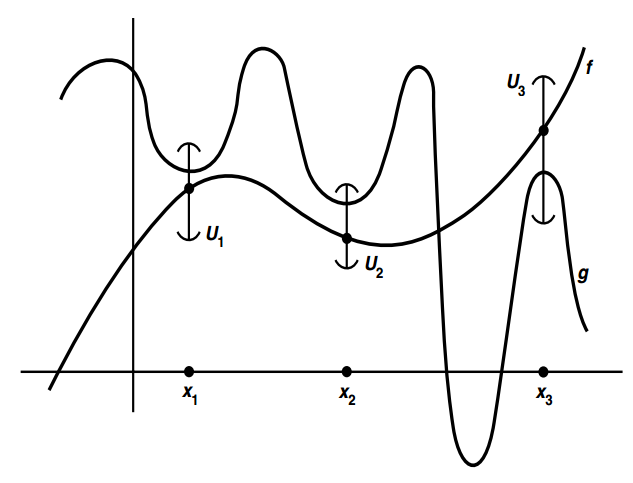
\includegraphics[scale = 0.4]{pointwise_convergence_topology.png}}
\end{minipage}
\caption{\footnotesize{\textbf{The function $g$ in neighborhood of $f$ in topology of pointwise convergence. \citep{munkres2000topology}}}}
\label{fig: pointwise_convergence_topology}
\end{figure}


\item \begin{remark} (\emph{\textbf{Basis of Point-Open Topology}})\\
The general \emph{basis element} for this topology is a \emph{finite intersection} of subbasis elements $S(x, U)$. Thus a typical \emph{\textbf{basis element}} about the function $f$ \emph{consists of all functions $g$ that are \underline{\textbf{``close"} to $f$ \textbf{at finitely many points}}}. Such a \emph{neighborhood} is illustrated in Figure \ref{fig: pointwise_convergence_topology}; it consists of all functions $g$ whose graphs \emph{intersect the three vertical intervals} pictured.
\end{remark}

\item \begin{remark}
\emph{\textbf{The topology of pointwise convergence on $Y^X$ is \underline{the product topology}}}. 

If we replace $X$ by $J$ and denote the general element of $J$ by $\alpha$ to make it look more familiar, then the set $S(\alpha, U)$ of all functions $x : J \rightarrow Y$
such that $x(\alpha) \in U$ is just the subset $\pi_{\alpha}^{-1}(U)$ of $Y^J$, which is \emph{the standard subbasis element} for the product topology.
\end{remark}

\item \begin{proposition} (\textbf{Pointwise Convergence Topology})\citep{munkres2000topology}\\
A sequence $f_n$ of functions \textbf{converges} to the function $f$ in the \textbf{topology of pointwise convergence} \textbf{if and only if} for \textbf{each} $x$ in $X$, the sequence $f_n(x)$ of \textbf{points of $Y$} converges to the point $f(x)$.
\end{proposition}


\item \begin{remark}
Compare the \emph{subbasis} of \emph{the point-open topology} on function space $Y^X$ and \emph{the weak topology} on space $X$
\begin{align*}
S(x, U) = \set{f:  f \in Y^X\text{ and }f(x) \in U} &\quad \text{\emph{point-open topology}}.\\
B(f, U) = \set{x:  x \in X\text{ and }f(x) \in U} &\quad \text{\emph{weak topology}}.
\end{align*}
\end{remark}

\item \begin{example} (\textbf{Pointwise Convergence Does Not Preserve Continuity})\\
Consider the space $\bR^I$, where $I = [0, 1]$. The sequence $(f_n)$ of continuous functions given by $f_n(x) = x^n$ \emph{converges} in the \emph{\textbf{topology of pointwise convergence}} to the function $f$ defined by
\begin{align*}
f(x) &=\left\{ 
\begin{array}{cc}
0 &\text{ for } 0 \le x < 1\\
1 &\text{ for } x = 1
\end{array}\right.,
\end{align*}
This example shows that the subspace $\cC(I, \bR)$ of continuous functions is \emph{\textbf{not closed}} in $\bR^I$
\emph{in the topology of pointwise convergence}. Note that $\cC(I, \bR)$  is \emph{\textbf{closed} in $\bR^I$ under \textbf{uniform topology}} due to \emph{Uniform Limit theorem}. 
\end{example}

\item \begin{definition} (\emph{\textbf{Topology of Compact Convergence}})\\
Let $(Y, d)$ be a \emph{metric space}; let $X$ be a \emph{topological space}. Given an element $f$ of $Y^X$, a \emph{\textbf{compact subspace}} $C$ of $X$, and a number $\epsilon > 0$, let $B_{C}(f, \epsilon)$ denote the set of all those elements $g$ of $Y^X$ for which
\begin{align*}
\sup\{d(f (x), g(x)): x \in C\} < \epsilon.
\end{align*}
The sets $B_{C}(f, \epsilon)$  form a \emph{\textbf{basis}} for a topology on $Y^X$. It is called the \underline{\emph{\textbf{topology of compact}}} \underline{\emph{\textbf{convergence}}} (or sometimes the ``\underline{\emph{\textbf{topology of uniform convergence on compact sets}}}").
\end{definition}

\item \begin{proposition} (\textbf{Topology of Uniform Convergence in Compact Sets}) \citep{munkres2000topology}\\
A sequence $f_n : X \rightarrow Y$ of functions converges to the function $f$ in the \textbf{topology of compact convergence} if and only if for \textbf{each compact subspace} $C$ of $X$, the sequence $f_n|_{C}$ converges \textbf{uniformly} to $f|_C$.
\end{proposition}

\item \begin{definition}
A space $X$ is said to be \underline{\emph{\textbf{compactly generated}}} if it satisfies the following condition: A set $A$ is \emph{\textbf{open}} in $X$ if $A \cap C$ is \emph{\textbf{open}} in $C$ for each \textbf{compact subspace} $C$ of $X$.
\end{definition}

\item \begin{lemma} \citep{munkres2000topology}\\
If $X$ is \textbf{locally compact}, or if $X$ satisfies \textbf{the first countability axiom}, then $X$ is \textbf{compactly generated}.
\end{lemma}

\item The crucial fact about compactly generated spaces is the following:
\begin{lemma} (\textbf{Continuous Extension on Compact Generated Space})  \citep{munkres2000topology}\\
If $X$ is compactly generated, then a function $f : X \rightarrow Y$ is \textbf{continuous} if for each \textbf{compact subspace} $C$ of X, the restricted function $f |_{C}$ is \textbf{continuous}.
\end{lemma}


\item \begin{theorem} (\textbf{$\cC(X, Y)$ on Compact Generated Space})  \citep{munkres2000topology}\\
Let $X$ be a \underline{\textbf{compactly generated space}}: let $(Y, d)$ be a metric space. Then $\cC(X, Y)$ is \underline{\textbf{closed}} in $Y^X$ in the \underline{\textbf{topology of compact convergence}}.
\end{theorem}


\item \begin{corollary} (\textbf{Compact Convergence Limit})  \citep{munkres2000topology}\\
Let $X$ be a \textbf{compactly generated space}; let $(Y, d)$ be a \textbf{metric} space. If a sequence of \textbf{continuous} functions $f_n : X \rightarrow Y$ converges to $f$ in the \textbf{topology of compact convergence}, then $f$ is \textbf{continuous}.
\end{corollary}

\item \begin{remark} (\emph{\textbf{Useful Topologies on $Y^X$}})
\begin{enumerate}
\item \underline{\emph{\textbf{Uniform Topology}}}: generated by the \emph{\textbf{basis}}
\begin{align*}
B_{U}(f, \epsilon) &= \set{g \in Y^X: \sup_{x\in X}\bar{d}(f(x), g(x)) < \epsilon }
\end{align*} It corresponds to \emph{\textbf{the uniform convergence}} of $f_n$ to $f$ in $Y^X$. $\cC(X, Y)$ is \emph{\textbf{closed}} in $Y^X$ under the \emph{uniform topology}, following \emph{the Uniform Limit Theorem}.

\item  \underline{\emph{\textbf{Topology of Pointwise Convergence}}}: generated by the \emph{\textbf{basis}}
\begin{align*}
B_{U_1 \xdotx{,} U_n}(x_1 \xdotx{,} x_n, \epsilon)  &= \bigcap_{i=1}^{n}S(x_i, U_i) \\
&= \set{f \in Y^X: f(x_1) \in U_1 \xdotx{,} f(x_n) \in U_n}, \quad   1 \le n < \infty.
\end{align*} It corresponds to \emph{\textbf{the pointwise convergence}} of $f_n$ to $f$ in $Y^X$. $\cC(X, Y)$ is \emph{\textbf{not closed}} in $Y^X$ under the \emph{topology of pointwise convergence}

\item \underline{\emph{\textbf{Topology of Compact Convergence}}}: generated by the \emph{\textbf{basis}}
\begin{align*}
B_{C}(f, \epsilon) &= \set{g \in Y^X: \sup_{x \in C}d(f (x), g(x)) < \epsilon }.
\end{align*} It corresponds to \emph{\textbf{the uniform convergence}} of $f_n$ to $f$ in $Y^X$ for $x \in C$. $\cC(X, Y)$ is \emph{\textbf{closed}} in $Y^X$ under the \emph{topology of compact convergence} \emph{\textbf{if $X$ is compactly generated}}.
\end{enumerate}
\end{remark}

\item \begin{theorem} (\textbf{Relationship between Topologies on $Y^X$}) \citep{munkres2000topology}\\
Let $X$ be a space; let $(Y, d)$ be a metric space. For the function space $Y^X$ , one has the following \textbf{inclusions of topologies}:
\begin{align*}
\text{\textbf{(uniform)}} \supseteq \text{\textbf{(compact convergence)}} \supseteq \text{\textbf{(pointwise convergence)}}.
\end{align*}
If $X$ is \textbf{compact}, the \textbf{first two} coincide, and if $X$ is \textbf{discrete}, the \textbf{second two} coincide.
\end{theorem}

\item \begin{remark}
Note that both \emph{uniform topology} and \emph{topology of compact convergence} rmade specific use of the metric $d$ for the space $Y$, i.e. it can only be defined when the image of function $Y$  is a metric space.

But \emph{\textbf{the topology of  pointwise convergence}} does \emph{not use the definition of metric} $d$ in $Y$. In fact, \emph{\textbf{it is defined for any image space $Y$}}.
\end{remark}


\item \begin{definition} (\emph{\textbf{Compact-Open Topology on Continuous Function Space}})\\
Let $X$ and $Y$ be topological spaces. If $C$ is a \emph{\textbf{compact subspace}} of $X$ and $U$ is an \emph{open} subset of $Y$, define
\begin{align*}
S(C,U) = \set{ f \in \cC(X, Y): f(C) \subseteq U}.
\end{align*}
The sets $S(C, U)$ form a \emph{\textbf{subbasis}} for a \emph{topology} on $\cC(X, Y)$ that is called \underline{\emph{\textbf{the compact-open}}} \underline{\emph{\textbf{topology}}}.
\end{definition}

\item \begin{proposition} (\textbf{Compact-Open on $\cC(X, Y)$ $=$ Compact Convergence}) \citep{munkres2000topology}\\
Let $X$ be a space and let $(Y, d)$ be a metric space. On the set $\cC(X, Y)$, the \textbf{compact-open topology} and the \textbf{topology of compact convergence} \textbf{coincide}.
\end{proposition}

\item \begin{corollary}(\textbf{Compact Convergence on $\cC(X, Y)$ Need Not $d$}) \citep{munkres2000topology}\\
Let $Y$ be a metric space. The \textbf{compact convergence topology} on $\cC(X, Y)$ does  \textbf{not} depend on the \textbf{metric} of $Y$. Therefore if $X$ is \textbf{compact}, the \textbf{uniform topology} on $\cC(X, Y)$ does not depend on the metric of $Y$.
\end{corollary}

\item \begin{remark} 
The fact that the definition of \emph{\textbf{the compact-open topology}} does not involve a \emph{\textbf{metric}} is just one of its useful features. 

Another is the fact that it satisfies the requirement of ``\emph{\textbf{joint continuity}}.” Roughly speaking, this means that the expression $f(x)$ is
\emph{continuous} not only in the \emph{single}``variable”  $x$, but is \emph{\textbf{continuous jointly} in \textbf{both} the $x$ and $f$} .
\end{remark}

\item \begin{theorem} (\textbf{Compact-Open Topology $\Rightarrow$ Joint Continuity for $x$ and $f$})\\
Let $X$ be \textbf{locally compact Hausdorff}; let $\cC(X, Y)$ have the \textbf{compact-open topology}. Then the map
\begin{align*}
e: X \times \cC(X, Y) \rightarrow Y
\end{align*}
defined by the equation
\begin{align*}
e(x, f) = f(x)
\end{align*}
is \textbf{continuous}. The map $e$ is called \underline{\textbf{the evaluation map}}.
\end{theorem}

\item \begin{definition}
Given a function $f : X \times Z \rightarrow Y$, there is a corresponding function $F : Z \rightarrow \cC(X, Y)$, defined by the equation
\begin{align*}
(F(z))(x) = f(x, z).
\end{align*}
Conversely, given $F : Z \rightarrow \cC(X, Y)$, this equation defines a corresponding function
$f : X \times Z \rightarrow Y$. We say that $F$ is the map of $Z$ into $\cC(X, Y)$ that is induced by $f$.
\end{definition}

\item \begin{proposition}
Let $X$ and $Y$ be spaces; give $\cC(X, Y)$ the \textbf{compact-open topology}. If $f: X \times Z \rightarrow Y$ is \textbf{continuous}, then \textbf{so is} the induced function $F : Z \rightarrow \cC(X, Y)$. The \textbf{converse} holds if $X$ is \textbf{locally compact Hausdorff}.
\end{proposition}

\item \begin{theorem} (\textbf{Ascoli's Theorem, General Version}). \citep{munkres2000topology} \\
Let $X$ be a space and let $(Y, d)$ be a \underline{\textbf{metric}} space. Give $\cC(X, Y)$ the \underline{\textbf{topology of compact}} \underline{\textbf{convergence}}; let $\cF$ be a subset of $\cC(X, Y)$.
\begin{enumerate}
\item If $\cF$ is \underline{\textbf{equicontinuous}} under $d$ and the set
\begin{align*}
F_{a} &= \set{f(a): f \in \cF}
\end{align*}
has \underline{\textbf{compact closure}} for each $a \in X$, then $\cF$ is \underline{\textbf{contained} in a \textbf{compact subspace}} of $\cC(X, Y)$.
\item  The \textbf{converse} holds if $X$ is \underline{\textbf{locally compact Hausdorff}}.
\end{enumerate}
\end{theorem}

\item \begin{remark} 
Compare with classical version, we see generalizations:
\begin{enumerate}
\item $X$ need not to be \emph{\textbf{compact}}; $\Rightarrow$ does not even need $X$ to be topological. $\Leftarrow$ holds when $X$ is \textbf{\emph{locally compact Hausdorff}}.
\item $\cC(X, Y)$ is under \emph{\textbf{compact-open topology}} which is \emph{\textbf{weaker}} than \emph{\textbf{uniform topology}}, i.e. we does not require convergence of sequence \emph{uniformly} but only \emph{uniformly in a compact subset}.
\item $\cF$ does not need to be \emph{\textbf{pointwise bounded}} under $d$. In other word, the set 
\begin{align*}
F_{a} &= \set{f(a): f \in \cF}
\end{align*} need not to be \emph{\textbf{bounded}} but need to have \emph{\textbf{compact closure}} for each $a \in X$. Note that for metric space $Y$, if $Y$ is finite dimensional, it is the same requirement as boundness. But compact closure is stronger than bounded.
\end{enumerate}
\end{remark}

\item \begin{proposition} (\textbf{Equicontinuity $+$ Pointwise Convergence $\Rightarrow$ Compact Convergence}) \citep{munkres2000topology}\\
Let $(Y, d)$ be a metric space; let $f_n : X \rightarrow Y$ be a sequence of \textbf{continuous} functions; let $f : X \rightarrow Y$ be a function (not necessarily continuous). Suppose $f_n$ converges to $f$ in the \textbf{topology of pointwise convergence}. If $\{f_n\}$ is \textbf{equicontinuous}, then $f$ is \textbf{continuous} and $f_n$ converges to $f$ in the \textbf{topology of compact convergence}.
\end{proposition}
\end{itemize}


\section{Compactness in Banach Space}
\begin{remark} (\emph{\textbf{Compactness in Function Space}})\\
The importance of \emph{\textbf{compactness}} in analysis is well-known, and the fact tha \emph{closed bounded sets} are \emph{compact} in \emph{finite dimensional spaces} lies at the heart of much of the analysis on these spaces. \emph{\textbf{Unfortunately}}, as we have seen, this is \emph{not true} in \emph{infinite dimensional spaces}.

There are \emph{\textbf{two main compactness results}} in \emph{function space}:
\begin{enumerate}
\item The \underline{\textbf{\emph{Ascoli's theorem}}}: Let $X$ be a \emph{compact Hausdorff space}; let $d$ denote either the square metric or the euclidean metric on $\bR^n$; give $\cC(X, \bR^n)$ the corresponding \textbf{\emph{uniform topology}}. \emph{A subspace $\srF$ of $\cC(X, \bR^n)$ is \textbf{compact} if and only if it is \underline{\textbf{closed}, \textbf{bounded}} under the \underline{\textbf{sup metric} $\rho$}, and \underline{\textbf{equicontinuous}} under $d$}.

\item The \underline{\textbf{\emph{Banach-Alaoglu theorem}}}: Let $X$ be a \emph{Banach space}. \emph{The \textbf{unit ball} in $X^{*}$, $\{f \in X^{*}: \norm{f}{}\le 1\}$ is \textbf{compact} in the \underline{\textbf{weak$^{*}$ topology}}}.

In this section we will show that a \emph{partial analogue} of this result can be obtained in \emph{\textbf{infinite dimensions}} if we adopt a \emph{weaker definition of the convergence} of a sequence than the usual definition.
\end{enumerate}


\end{remark}
\subsection{Strong and Weak Convergence}
\begin{itemize}
\item \begin{definition} (\emph{\textbf{Strong Convergence}}). \citep{kreyszig1989introductory}\\
A sequence $(x_n)$ in a normed space $X$ is said to be \underline{\emph{\textbf{strongly convergent}}} (or \emph{\textbf{convergent \underline{in the norm}}}) if
there is  an $x \in X$ such that
\begin{align*}
\lim\limits_{n\rightarrow \infty} \norm{x_n - x}{} = 0.
\end{align*}
This is written $\lim\limits_{n\rightarrow \infty}x_n = x$ or simply $x_n \rightarrow x$ is called \emph{the \textbf{strong limit} of $(x_n)$}, and we say that $(x_n)$ \emph{converges \textbf{strongly} to $x$}. 
\end{definition}

\item \begin{definition} (\emph{\textbf{Weak Convergence}}). \citep{kreyszig1989introductory}\\
A sequence $(x_n)$ in a normed space $X$ is said to be \underline{\emph{\textbf{weakly convergent}}} if there is an $x \in X$ such that \emph{for \textbf{every}} $f \in X^{*}$,
\begin{align*}
\lim\limits_{n\rightarrow \infty} f(x_n) = f(x).
\end{align*}
This is written $x_n \stackrel{w}{\rightarrow} x$ or $x_n \rightharpoonup x$. The element $x$ is called \emph{\textbf{the weak limit} of $(x_n)$}, and we say
that \underline{$(x_n)$ \emph{\textbf{converges weakly} to $x$.}}
\end{definition}

\item \begin{remark}
For weak convergence, we see it as convergence of \emph{real numbers} $s_n = f(x_n)$ in $\bR$.
\end{remark}

\item \begin{remark} (\emph{\textbf{Weak Convergence Analysis is Common}})\\
\emph{\textbf{Weak convergence}} has various applications throughout analysis (for instance, in the \emph{calculus of variations}, \emph{the general theory of
differential equations} and \emph{probability theory}). 

The concept illustrates \emph{\textbf{a basic principle of functional analysis}}, namely, the fact that \underline{\textbf{\emph{the investigation of spaces is often related to that of their dual spaces}}}, i.e. \emph{probing a variable by using a test functional}.
\end{remark}

\item \begin{remark}
In \emph{Hilbert space} $\cH$, we say $x_n \stackrel{w}{\rightarrow} x$ if there exists an $x\in \cH$ such that for all $y \in \cH$
\begin{align*}
\lim\limits_{n\rightarrow \infty} \inn{x_n}{y} = \inn{x}{y}.
\end{align*} Note that given a set of orthonormal basis $(e_n)$, we have $f(e_n):= \inn{e_n}{y}$ and from Bessel inequality
\begin{align*}
\sum_{n=1}^{\infty}\abs{\inn{e_n}{y}}^2 \le \norm{y}{}^2 < \infty \\
\Rightarrow \lim\limits_{n\rightarrow \infty}\abs{\inn{e_n}{y}} \rightarrow 0 \\
\Rightarrow e_n \stackrel{w}{\rightarrow} 0.
\end{align*} But $\norm{e_n - e_{m}}{} \not\rightarrow 0$, $(e_n)$ does not converge in norm (strongly).
\end{remark}

\item \begin{lemma}  (\textbf{Weak Convergence}).\\
Let $(x_n)$ be a \textbf{weakly convergent} sequence in a normed space $X$, say, $x_n \stackrel{w}{\rightarrow} x$. Then:
\begin{enumerate}
\item The weak limit $x$ of $(x_n)$ is \textbf{unique}.
\item Every \textbf{subsequence} of $(x_n)$ converges weakly to $x$.
\item The sequence $(\norm{x_n}{})$ is \textbf{bounded}.
\end{enumerate}
\end{lemma}

\item \begin{proposition} (\textbf{Strong and Weak Convergence}).  \citep{kreyszig1989introductory}\\
Let $(x_n)$ be a sequence in a normed space $X$. Then:
\begin{enumerate}
\item \textbf{Strong convergence} implies \textbf{weak convergence} with the same limit.
\item The converse of (1) is \textbf{not} generally true.
\item If $\text{dim }X < \infty$, then \textbf{weak convergence} implies\textbf{ strong convergence}.
\end{enumerate}
\end{proposition}

\item \begin{remark}
From above, we see that in \emph{\textbf{finite dimensional normed spaces}} the distinction between \emph{\textbf{strong}} and \emph{\textbf{weak convergence}} disappears completely. 
\end{remark}

\end{itemize}
\subsection{Weak Topology}
\begin{itemize}
\item \begin{remark}
The weak convergence, $x_n \stackrel{w}{\rightarrow} x$, can be considered as \emph{convergence of net $\set{x_n}_{n=1}^{\infty}$ in the \textbf{weak topology}}.
\end{remark}

\item \begin{definition} (\textbf{\emph{Weak Topology on a Set $S$}})  \citep{reed1980methods}\\
Let $\cF$ be a family of functions from a set $S$ to a topological vector space $(X, \srT)$. The \emph{\textbf{$\cF$-weak} (or simply \textbf{weak}) \textbf{topology}} on $S$ is the weakest topology for which \emph{\textbf{all the functions} $f \in \cF$ are \textbf{continuous}}.
\end{definition}

\item \begin{remark} (\emph{\textbf{Construction of Weak Topology}}) \citep{reed1980methods} \\
To construct a \emph{\textbf{$\cF$-weak topology}} on $S$, we take the family of \emph{all \underline{\textbf{finite intersections}} of sets} of the form $f^{-1}(U)$ where $f \in \cF$ and $U \in \srT$. The collections of these finite intersections of sets \emph{form \textbf{a basis} of \textbf{the $\cF$-weak topology}}.

In other word, \emph{\textbf{the subbasis}} for the \emph{$\cF$-weak topology} on $S$ is of form 
\begin{align*}
\srS = \set{f^{-1}(U):  f \in \srF, \text{ and }  U \in \srT}
\end{align*}
And the basis of $\srT$
\begin{align*}
\srB &= \set{f_1^{-1}(U_1) \xdotx{\cap} f_k^{-1}(U_k): f_1 \xdotx{,} f_k \in \srF, \;\; U_1 \xdotx{,} U_k \in \srT, \;1 \le k < \infty}\\
B \in \srB \Rightarrow B &= \set{x: f_1(x) \in U_1 \xdotx{,} f_k(x) \in U_k},\; 1 \le k < \infty \\
&= \set{x: (f_1(x) \xdotx{,} f_k(x)) \in U}.
\end{align*} The basis element is called a \underline{\emph{\textbf{$k$-dimensional cylinder set}}}.
\end{remark}

\item \begin{remark}
Given a topology  on $Y$ and a family of functions in $Y^X= \set{f: X\rightarrow Y}$, $\srF$-weak topolgy is \emph{\textbf{a natural topology}} on $X$ without additional information. 

A product topology on $Y^{\omega}$ can be seen as a $\srF$-weak topology when $\srF = \{\pi_{\alpha}: \prod_{i}Y_i \rightarrow Y_{\alpha} \}$.
\end{remark}

\item \begin{remark}
A set $S$ equipped with \emph{$\cF$-weak topology} \emph{\textbf{has little knowledge on itself besides the output of functions}} $f \in \cF$ from a family $\cF$. The induced topology through a family of functions thus does not tell much besides  the behavior of its output. 

For instance, $S$ is the space of hidden states, $\cF = \set{f_1 \xdotx{,} f_n} \subset 2^{S}$ is a series of binary statistical tests, the weak topology on $S$ \emph{partition the domain according to the output of each test}. 
\end{remark}

\item \begin{remark}
By construction,  the \emph{\textbf{neighborhood base}} of each point $x \in S$ under the $\cF$-weak topology is contained in the pre-images  $\{f_{n}^{-1}(U_{n})\}$ for \emph{\textbf{finitely many}} of $(f_n) \in \cF$.
\end{remark}


\item \begin{definition} (\textbf{\emph{Weak Topology on Banach Space}})\\
Let $X$ be a \emph{\textbf{Banach space}} with dual space $X^{*}$. The \underline{\emph{\textbf{weak topology}} on $X$} is \emph{the weakest topology} on $X$ so that \emph{$f(x)$ is \textbf{continuous} \textbf{for all} $f \in X^{*}$}.
\end{definition}

\item \begin{remark}
For infinite dimensional Banach spaces, \emph{\textbf{the weak topology does not arise from a metric}}. This is one of the main reasons we have introduced topological spaces.
\end{remark}

\item \begin{remark}
Thus a \emph{\textbf{neighborhood} base at zero} for \emph{\textbf{the weak topology}} is given by the sets
of the form
\begin{align*}
N(f_1 \xdotx{,} f_n; \epsilon) &= \set{x: \abs{f_{j}(x)} <\epsilon; \; j= 1 \xdotx{,} n}
\end{align*}
that is, neighborhoods of zero contain \emph{\textbf{cylinders} with \textbf{finite-dimensional} open bases}. A net $\{x_{\alpha}\}$ converges \emph{weakly} to $x$, written $x_\alpha \stackrel{w}{\rightarrow} x$, if and only if $f(x_{\alpha}) \rightarrow f(x)$ for all $f \in X^{*}$.
\end{remark}



\item \begin{proposition} \citep{reed1980methods}
\begin{enumerate}
\item The weak topology is \textbf{weaker} than \textbf{the norm topology}, that is, every weakly open set is norm open.
\item Every \textbf{weakly convergent} sequence is \textbf{norm bounded}.
\item The weak topology is a \textbf{Hausdorff} topology.
\end{enumerate}
\end{proposition}


\item \begin{proposition} (\textbf{Weak Topology on Hilbert Space}) \citep{reed1980methods}\\
Let $\cH$ be a \textbf{Hilbert space}. Let $\set{\varphi_{\alpha}}_{\alpha \in I}$ be an \textbf{orthonormal basis} for $\cH$. Given a sequence $\psi_{n} \in \cH$, let 
\begin{align*}
\psi_{n}^{(\alpha)}= \inn{\psi_n}{\varphi_{\alpha}}
\end{align*}
be the coordinates of $\psi_n$. Then $\psi_n \rightarrow \psi$  in the \textbf{weak topology} (or  $\psi_n \stackrel{w}{\rightarrow} \psi$) \textbf{if and only if}
\begin{enumerate}
\item $\psi_{n}^{(\alpha)} \rightarrow \psi^{(\alpha)}$ for each $\alpha$; and
\item $\norm{\psi_n}{}$ is \textbf{bounded}.
\end{enumerate}
\end{proposition}
\begin{proof}
Suppose $\psi_n \stackrel{w}{\rightarrow} \psi$; then (1) follows by  definition and (2) comes from the fact that \emph{every weakly convergent sequence is norm bounded}. 

On the other hand, let (1) and (2) hold and let $\cF \subset \cH$ be the subspace of \emph{finite linear combinations} of the $\varphi_{\alpha}$. By (1), 
$\inn{\psi_n}{\varphi_{\alpha}} \rightarrow \inn{\psi}{\varphi_{\alpha}}$ if $\varphi \in \cF$. Using the fact that $\cF$ is dense, (2), and an $\epsilon/3$ argument, the weak convergence follows. \qed
\end{proof}

\item \begin{proposition} (\textbf{Weak Topology of $\cC(X)$ on Compact Hausdorff Space}) \citep{reed1980methods}\\
Let $X$ be a \textbf{compact Hausdorff} space and consider the \textbf{weak topology on} $\cC(X)$ (i.e. $\cC(X, \bR)$). Let $\{f_n\}$ be a sequence in $\cC(X)$. Then $f_n \rightarrow f$  in the \textbf{weak topology} (or  $f_n \stackrel{w}{\rightarrow} f$) \textbf{if and only if}
\begin{enumerate}
\item $f_{n}(x) \rightarrow f(x)$ for each $x \in X$; and
\item $\norm{f_n}{}$ is \textbf{bounded}.
\end{enumerate}
\end{proposition}
\begin{proof}
For if  $f_n \stackrel{w}{\rightarrow} f$, then (1) holds since $f \rightarrow f(x)$ is an element of $\cC(X)^{*}$ and (2) 
comes from  the fact that \emph{every weakly convergent sequence is norm bounded}.  

On the other hand, if (1) and (2) hold,  then 
\begin{align*}
\abs{f_n(x)} \le \sup_{n}\norm{f_n}{\infty}
\end{align*}
which is $L^1$ with respect to any \emph{Baire measure} $\mu$. Thus, by the \emph{dominated convergence theorem}, for any $\mu \in \cM_{+}(X)$, $\int f_n d\mu \rightarrow \int f d\mu$. Since any $\lambda \in \cM(X) = \cC(X)^{*}$ is a \emph{finite linear combination} of measures in $\cM_{+}(X)$, we conclude that $f_n \rightarrow f$ weakly. \qed
\end{proof}


\item \begin{proposition} (\textbf{Banach Space Weak Continuity $=$ Norm Continuity}) \citep{reed1980methods}\\
A linear functional $f$ on a \textbf{Banach space} is \textbf{weakly continuous} \textbf{if and only if} it is \textbf{norm continuous}.
\end{proposition}

\end{itemize}

\subsection{Weak$^{*}$  Topology}
\begin{itemize}
\item \begin{definition}  (\textbf{\emph{Weak$^{*}$ Topology on Banach Space}})\\
Let $X$ be a \emph{normed vector space} and $X^{*}$ be its dual space. The \underline{\emph{\textbf{weak$^{*}$ topology}} on $X^{*}$} is \emph{the weakest topology} on $X^{*}$ so that \emph{$f(x)$ is \textbf{continuous} \textbf{for all} $x \in X$}.
\end{definition}

\item \begin{remark}
\emph{\textbf{The weak$^{*}$ topology}} can be considered as a topology induced by $x \in X$ on dual space $X^{*}$, i.e. a topology on functional space on $X$ induced by point in $X$. 

In fact, \underline{\emph{\textbf{the weak$^{*}$ topology}} is \emph{the \textbf{topology} of \textbf{pointwise convergence}}}:
\begin{align*}
f_{\alpha} \rightarrow  f \quad \Leftrightarrow \quad f_{\alpha}(x) \rightarrow  f(x) \text{ for all }x \in X.
\end{align*} Moreover, \underline{\emph{\textbf{the weak$^{*}$ topology}} is \emph{the \textbf{product topology} on product space $\bR^X$}}.
\end{remark}

\item \begin{definition} (\emph{\textbf{$Y$-Weak Topology  $\sigma(X, Y)$}})\\
Let $X$ be a \emph{vector space} and let $Y$ be a \emph{family of \textbf{linear functionals}} on $X$ which \emph{\textbf{separates points}} of $X$. That is, for any $x_1 \neq x_2$ in $X$, there exists a $f \in Y$ so that $f(x_1) \neq f(x_2)$. Then \underline{\emph{\textbf{the $Y$-weak topology on $X$}}, written $\sigma(X, Y)$}, is \emph{the weakest topology} on $X$ for which all the \emph{functionals} in $Y$ are \emph{continuous}. 
\end{definition}

\item \begin{remark}
\emph{$Y$-weak topology} $\sigma(X, Y)$ is \emph{the $\srF$-weak topology} when \emph{domain} of  $\srF$ is a \emph{vector space} and $\srF$ is a family of \emph{linear functionals}.
\end{remark}

\item \begin{remark}
Because $Y$ is assumed to \emph{separate points}, $\sigma(X, Y)$ is \emph{a \textbf{Hausdorff topology}} on $X$.  Note that
\begin{enumerate}
\item \emph{the weak topology} on $X$ is \emph{the $\sigma(X, X^{*})$ topology}
\item \emph{the weak$^{*}$ topology} on $X^{*}$ is \emph{the $\sigma(X^{*}, X)$ topology}
\end{enumerate}

The \emph{$\sigma(X, Y)$ topology} \emph{depends} only on \emph{\textbf{the vector space generated by }$Y$} so we henceforth suppose  that  \emph{$Y$ is a vector space}. 
\end{remark}


\item \begin{remark}
Notice that \emph{\textbf{the weak$^{*}$ topology} is even \textbf{weaker} than \textbf{the weak topology}}.
\begin{align*}
 \text{\emph{\textbf{the norm topology}}} \; \subset \; \text{\emph{\textbf{the weak topology}}} \; \subseteq \; \text{\emph{\textbf{the weak$^{*}$ topology}}}
\end{align*}
\end{remark}

\item \begin{remark}
As one might expect, \underline{$X$ is \emph{\textbf{reflexive}}} if and only if the \emph{\textbf{weak}} and \emph{\textbf{weak$^{*}$ topologies}} \underline{\emph{\textbf{coincide}}}, and many \emph{characterizations} of \emph{reflexivity} depend on relations involving the \emph{weak} and \emph{weak$^{*}$ topologies}.
\end{remark}

\item \begin{proposition} (\textbf{$\sigma(X, Y)$ Topology $=$ Pointwise Convergence Topology on $X$}) \citep{reed1980methods} \\
The $\sigma(X, Y)$-\textbf{continuous} linear functionals on $X$ are \textbf{precisely} $Y$, in particular the only \textbf{weak$^{*}$ continuous functionals} on $X^{*}$ are  the \textbf{elements} of $X$. 
\end{proposition}

\item \begin{theorem} (\textbf{The Banach-Alaoglu Theorem}) \citep{reed1980methods}\\
 Let $X^{*}$ be the dual of some Banach space, $X$. Then \textbf{the unit ball} in $X^{*}$, $\set{f \in X^{*}: \norm{f}{}\le 1}$ is \underline{\textbf{compact}} in the \underline{\textbf{weak$^{*}$ topology}}.
\end{theorem}

\item \begin{corollary} (\textbf{The Banach-Alaoglu Theorem, Sequential Version}) \citep{rynne2007linear}\\
If $X$ is \textbf{separable} and $\set{f_n}$ is a \textbf{bounded} sequence in $X^{*}$, then  $\set{f_n}$ has a \textbf{\underline{weak$^{*}$ convergent} \underline{subsequence}}.
\end{corollary}

\item \begin{theorem}(\textbf{Kakutani's Theorem}) \citep{rynne2007linear}\\
$X$ is \textbf{reflexive} Banach space \underline{\textbf{if and only if}} \textbf{the unit ball} in $X$, $\set{x \in X: \norm{x}{}\le 1}$ is \underline{\textbf{compact}} in the \underline{\textbf{weak topology}}.
\end{theorem}

\item \begin{corollary} \citep{rynne2007linear}\\
If $X$ is \textbf{reflexive} Banach space and $\{x_n\}$ is a \textbf{bounded} sequence in $X$, then $\{x_n\}$ has a \textbf{\underline{weakly convergent subsequence}}.
\end{corollary}

\item \begin{corollary}\citep{rynne2007linear}\\
If $X$ is \textbf{reflexive} Banach space and $M \subseteq X$ is \underline{\textbf{bounded}, \textbf{closed} and \textbf{convex}}, then any sequence
in $M$ has a \textbf{subsequence} which is \textbf{weakly convergent} to an element of $M$.
\end{corollary}

\item \begin{exercise}\citep{rynne2007linear}\\
Suppose that $X$ is \textbf{reflexive} Banach space, $M$ is a \underline{\textbf{closed}, \textbf{convex} subset} of $X$, and
$y \in X \setminus M$.  Show that there is a point $y_M \in M$ such that
\begin{align*}
y - y_M = \inf\set{y- x: x \in M}.
\end{align*}
Show that this result is \textbf{not true} if the assumption that $M$ is \textbf{convex} is omitted.
\end{exercise}

\item \begin{example} (\emph{\textbf{Convergence in Distribution}})\\
\underline{\emph{\textbf{Convergence in distribution}}} is also called \underline{\emph{\textbf{weak convergence}}} in probability theory \citep{folland2013real}. In functional analysis, however, \emph{\textbf{weak convergence}} is actually reserved for a different mode of convergence, while \emph{\textbf{the convergence in distribution}} is \emph{\textbf{the weak$^*$ convergence}} on $\cM(X)$.

In general, it is actually \emph{\textbf{not} a mode of \textbf{convergence of functions} $f_n$ \textbf{itself}} but instead is \underline{\emph{the \textbf{convergence} of \textbf{bounded linear functionals}}} $\int f d\mu_n$. Equivalently, it is \emph{the \textbf{convergence of measures} $F_n$ on $\srB(\bR)$}.

\begin{align*}
 \text{weak convergence} && \int f_n d\mu \rightarrow \int f d\mu, \quad \forall \mu \in \cM(X), \\
\text{convergence in distribution}  &&  \int f d\mu_n \rightarrow \int f d\mu, \quad \forall f \in \cC_{0}(X)
\end{align*}

\begin{definition} (\emph{\textbf{Cumulative Distribution Function}}) \citep{van2000asymptotic} \\
Let $(\Omega,\srF, \mu)$ be a probability space. Given any real-valued measurable function $\xi : \Omega \rightarrow \bR$, we define the \emph{\textbf{cumulative distribution function}} $F : \bR \rightarrow [0, \infty]$ of $\xi$ to be the function
\begin{align*}
F_{\xi}(\lambda) :=  \mu\paren{\set{x \in  X : \xi(x) \le \lambda}} = \int_{X} \ind{\xi(x) \le \lambda}d\mu(x).
\end{align*}
\end{definition}

\begin{definition}  (\emph{\textbf{Converge in Distribution}}) \citep{van2000asymptotic}\\
Let $\xi_n : \Omega \rightarrow \bR$ be a sequence of real-valued \emph{measurable functions}, and $\xi: \Omega \rightarrow \bR$ be another measurable function. We say that $\xi_n$ \underline{\emph{\textbf{converges in distribution}}} to $\xi$ if \emph{the cumulative distribution function} $F_n(\lambda)$ of $\xi_n$
\underline{\emph{\textbf{converges pointwise}}} to the cumulative distribution function $F(\lambda)$ of $\xi$ at all $\lambda \in  \bR$ for which $F$ is continuous. Denoted as $\xi_{n}\stackrel{F}{\rightarrow} \xi$ or \underline{$\xi_{n}\stackrel{d}{\rightarrow} \xi$} or \underline{$\xi_n \rightsquigarrow \xi$}. 
\begin{align*}
\xi_{n}\stackrel{d}{\rightarrow} \xi \; \Leftrightarrow \; F_n(\lambda) \rightarrow F(\lambda), \text{ for all }\lambda \in \bR
\end{align*}
\end{definition}

\begin{theorem} (\textbf{The Portmanteau Theorem}).  \citep{van2000asymptotic}\\
 The following statements are equivalent.
 \begin{enumerate}
 \item $X_n \rightsquigarrow X$.
 \item $\E{}{h(X_n)} \rightarrow \E{}{h(X)}$ for all \textbf{continuous functions} $h: \bR^d \rightarrow \bR$ that are non-zero only on a \textbf{closed} and \textbf{bounded} set.
 \item $\E{}{h(X_n)} \rightarrow \E{}{h(X)}$ for all \textbf{bounded continuous functions} $h: \bR^d \rightarrow \bR$.
 \item $\E{}{h(X_n)} \rightarrow \E{}{h(X)}$ for all \textbf{bounded measurable functions} $h: \bR^d \rightarrow \bR$ for which $\bP(X \in \{x: h\text{ is continuous at }x\})=1$.
 \end{enumerate}
\end{theorem}

We can reformulate the definition of \emph{convergence in distribution} as below:
\begin{definition} \citep{wellner2013weak}\\
Let $(\cX, d)$ be a \emph{metric space}, and $(\cX, \srB)$ be \emph{a measurable space}, where $\srB$ is \emph{\textbf{the Borel $\sigma$-field on $\cX$}}, the smallest $\sigma$-field containing \emph{all the open balls} (as the basis of \emph{metric topology} on $\cX$). Let $\{\cP_n \}$ and $\cP$ be \emph{\textbf{Borel probability measures}} on $(\cX, \srB)$.

Then the sequence $\cP_n$ \underline{\emph{\textbf{converges in distribution}}} to $\cP$, which we write as $\cP_n \rightsquigarrow \cP$, if and only if
\begin{align*}
\int_{\Omega} f d\cP_n \rightarrow \int_{\Omega} f d\cP, \quad \text{ for all } f \in \cC_{b}(\cX).
\end{align*}
Here $\cC_{b}(\cX)$ denotes the set of \emph{all \textbf{bounded}, \textbf{continuous}, real functions on $\cX$}.
\end{definition} 
We can see that \underline{\emph{\textbf{the convergence in distribution}} is actually \emph{\textbf{a weak$^{*}$ convergence}}}. That is, it is \emph{\textbf{the weak convergence}} of  \emph{\textbf{bounded linear functionals}} $I_{\cP_n} \stackrel{w^{*}}{\rightarrow} I_{\cP}$ on \emph{the space of all probability measures} $\cP(\cX) \simeq (\cC_{b}(\cX))^{*}$ on $(\cX, \srB)$ where 
\begin{align*}
I_{\cP}: f \mapsto \int_{\Omega} f d\cP.
\end{align*} Note that the $I_{\cP_n} \stackrel{w^{*}}{\rightarrow} I_{\cP}$ is equivalent to $I_{\cP_n}(f) \rightarrow I_{\cP}(f)$ \emph{for all $f \in  \cC_{b}(\cX)$}.

%It also defines \emph{\textbf{a weak topology}} on $\cP(\Omega)$, the set of \emph{all probability measures} defined on measurable space $(\Omega, \srF)$. 
%Here $P_n \stackrel{w}{\rightarrow} P$ if and only if the cumulative distribution function $F_n(\lambda) \rightarrow F(\lambda)$ for all points $\lambda \in \bR$ at which $F$ is continuous.
\end{example}
\end{itemize}



\newpage
\bibliographystyle{plainnat}
\bibliography{reference.bib}
\end{document}